\subsection{Aplicação Fábrica: Registo de Ponto}
\subsubsection*{Descrição do caso de uso}
No registo do ponto, espera-se que utilizador entre na página e indique apenas o seu ID. A informação sobre a data e hora do registo deve ser automaticamente definida pelo sistema. 

\begin{figure}[H] 
	\begin{center}
		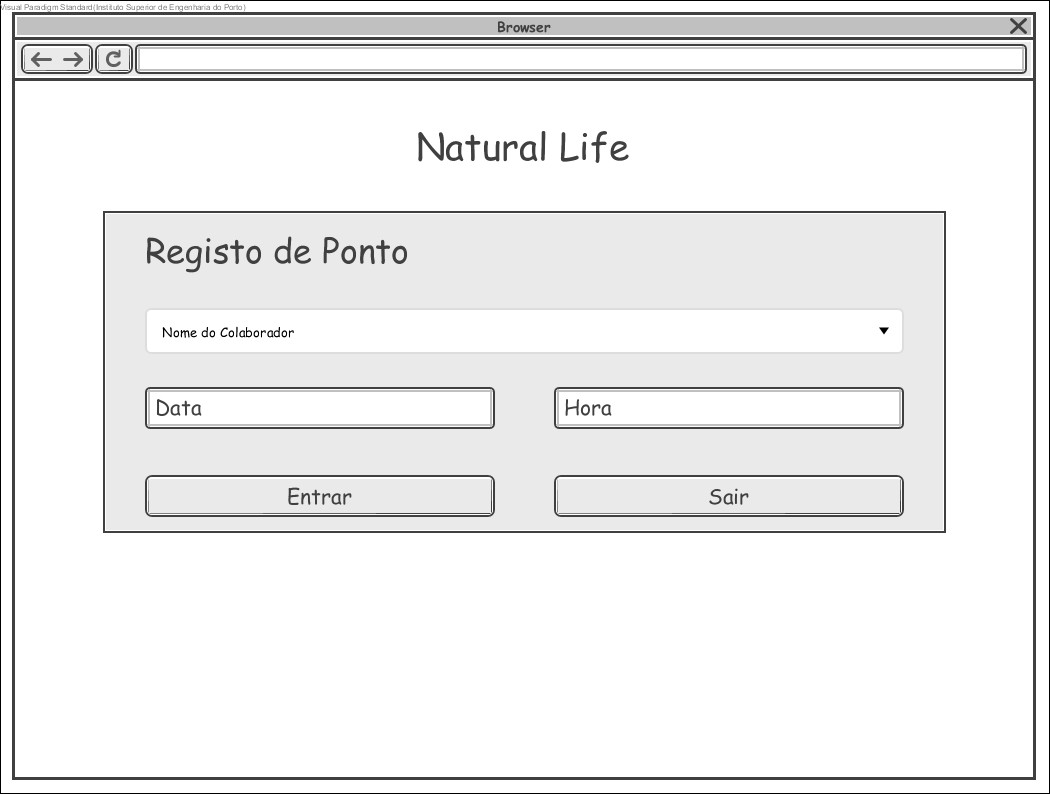
\includegraphics[width=0.60\textwidth,keepaspectratio]{figuras/Diagramas_vp/DI_Fabrica_1_Marcar_Ponto.jpg}
		\caption{Modelo do formulário do registo do ponto}
		\label{fig:di_ponto} 
	\end{center}
\end{figure}

\subsubsection*{Fluxo do caso de uso}
O caso de uso inicia-se com a abertura da página do registo de ponto. É apresentado o formulário com a data e hora previamente preenchidas. O utilizador tem de indicar o seu ID numa lista de dropdown. Após indicar o seu ID precisona o botão "Entrada" ou "Saída" conforme se esta a indicar o horario de entrada ou saída, respetivamente. Ambos os botões executam a submissão do formulário. Após o registo é apresentada uma mensagem ao utilizador


\begin{figure}[H] 
	\begin{center}
		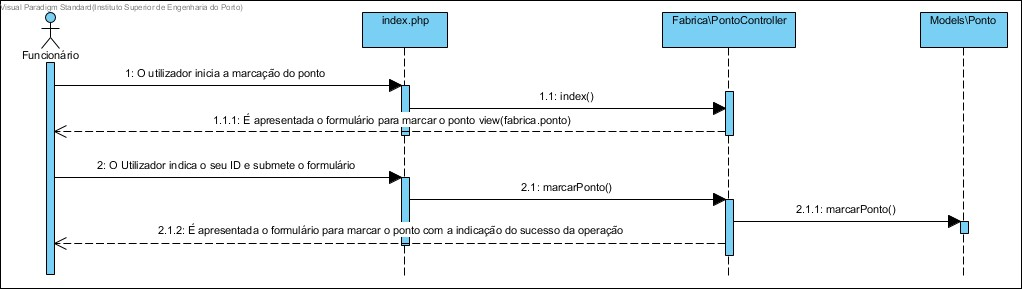
\includegraphics[width=\textwidth,keepaspectratio]{figuras/Diagramas_vp/SD_Fabrica_1_Marcar_Ponto.jpg}
		\caption{Diagrama de sequência marcar ponto}
		\label{fig:sd_ponto} 
	\end{center}
\end{figure}